% Adapted from LaTeX-examples-master/tikz/triangle-inscribed-circle.
% TeX Live 2025 draws a circle through the returned tangent point, so this
% fixture avoids the legacy [R] draw syntax from the original source.
\documentclass[border=3pt]{standalone}
\usepackage{tikz}
\usepackage{tkz-euclide}

\begin{document}
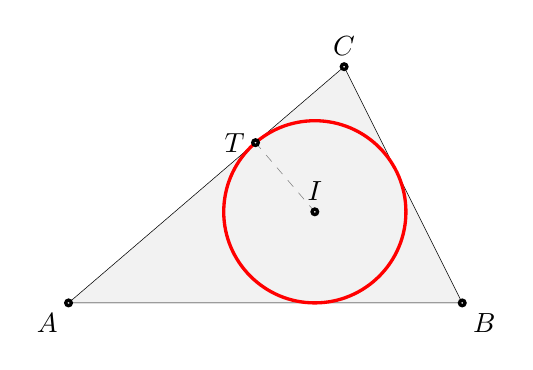
\begin{tikzpicture}[very thick]
  \tkzDefPoints{0/0/A,5/0/B,3.5/3/C}
  \tkzDrawPolygon[fill=gray!10](A,B,C)

  \tkzDefCircle[in,/tikz/overlay](A,B,C)\tkzGetPoints{I}{T}\tkzGetLength{rIN}
  \tkzDrawCircle[color=red,very thick](I,T)
  \tkzDrawSegments[dashed,gray](I,T)

  \tkzDrawPoints(A,B,C,I,T)
  \tkzLabelPoints[below left](A)
  \tkzLabelPoints[below right](B)
  \tkzLabelPoints[above](C)
  \tkzLabelPoint[above](I){$I$}
  \tkzLabelPoint[left](T){$T$}
\end{tikzpicture}
\end{document}
